\section{Results}
\label{sec:results}

The analysis covers a snapshot of the results database frozen on 16 October
2026 (\SnapshotRunCount{} ladder attempts, run identifiers up to
\SnapshotMaxRunId{}), of which \NValid{} runs are valid. The agents were
started inside the benchmark directory and were not sandboxed, and an audit of
the trajectories found \NEscapedRuns{} valid runs whose trajectory reads, lists, or searches files
outside their working copy, such as canonical task files, other runs, or hidden
tests. We call these \emph{escaped} runs. Fourteen of them come from the two Gemini arms and the rest from the two Grok
arms. We exclude them, which
leaves \NValidNoEsc{} runs, and report on this subset unless stated otherwise. Including them leaves
the planted-function results essentially unchanged (loose-rung drift of
\GoneLooseDriftFrac{} and \GtwoLooseDriftFrac{}, against \GoneScopedDriftFrac{}
and \GtwoScopedDriftFrac{} scoped and \GoneVagueDriftFrac{} and
\GtwoVagueDriftFrac{} vague); it does change one broader count, since three
generation-1 scoped runs that edited test files are among the excluded runs.
Table~\ref{tab:coverage} in Appendix~\ref{app:coverage} gives per-arm
coverage. Generation~1 covers the seven \emph{core} domains with every arm;
generation~2 covers all \NDomains{} domains, with Gemini~3.8 incomplete.
Almost every run passed every visible and hidden test at every rung
(Table~\ref{tab:ladder}); the
differences lie in what else the agents changed.

\begin{table*}[t]
\centering
\small
\caption{Outcomes by prompt rung, excluding escaped runs. \emph{Planted}: the
run edited at least one of the four planted functions (our primary drift
measure). \emph{Any out-of-scope}: the run edited a planted function, another
non-target function, a test file, or added a file. \emph{Test edits} is the
subset that changed or added test files. \emph{Pass gap}: visible pass minus
hidden pass, in percentage points.}
\label{tab:ladder}
\begin{tabular}{@{}llrrrrrrr@{}}
\toprule
Gen. & Rung & $n$ & Visible pass & Hidden pass & Pass gap & Planted & Any out-of-scope & Test edits \\
\midrule
1 & Scoped & \LgGoneScopedN & \LgGoneScopedVisiblePassPct & \LgGoneScopedHiddenPassPct & \LgGoneScopedPassGapPct & \ScGoneScopedPlantedPct & \ScGoneScopedAnyOosPct & \ScGoneScopedTestEditPct \\
  & Loose  & \LgGoneLooseN & \LgGoneLooseVisiblePassPct & \LgGoneLooseHiddenPassPct & \LgGoneLoosePassGapPct & \ScGoneLoosePlantedPct  & \ScGoneLooseAnyOosPct  & \ScGoneLooseTestEditPct \\
  & Vague  & \LgGoneVagueN & \LgGoneVagueVisiblePassPct & \LgGoneVagueHiddenPassPct & \LgGoneVaguePassGapPct & \ScGoneVaguePlantedPct  & \ScGoneVagueAnyOosPct  & \ScGoneVagueTestEditPct \\
\midrule
2 & Scoped & \LgGtwoScopedN & \LgGtwoScopedVisiblePassPct & \LgGtwoScopedHiddenPassPct & \LgGtwoScopedPassGapPct & \ScGtwoScopedPlantedPct & \ScGtwoScopedAnyOosPct & \ScGtwoScopedTestEditPct \\
  & Loose  & \LgGtwoLooseN & \LgGtwoLooseVisiblePassPct & \LgGtwoLooseHiddenPassPct & \LgGtwoLoosePassGapPct & \ScGtwoLoosePlantedPct  & \ScGtwoLooseAnyOosPct  & \ScGtwoLooseTestEditPct \\
  & Vague  & \LgGtwoVagueN & \LgGtwoVagueVisiblePassPct & \LgGtwoVagueHiddenPassPct & \LgGtwoVaguePassGapPct & \ScGtwoVaguePlantedPct  & \ScGtwoVagueAnyOosPct  & \ScGtwoVagueTestEditPct \\
\bottomrule
\end{tabular}
\end{table*}

\subsection{RQ1: How does the wording of a request affect drift?}
\label{sec:rq1}

In generation~1, \ScGoneLoosePlantedFrac{} loose-rung runs edited a planted
function (\ScGoneLoosePlantedPct{}, 95\% CI \ScGoneLoosePlantedCiLowPct{} to
\ScGoneLoosePlantedCiHighPct{}), against \ScGoneScopedPlantedFrac{} under the
scoped prompt and \ScGoneVaguePlantedFrac{} under the vague prompt.
Generation~2 reproduces the pattern: \ScGtwoLoosePlantedFrac{} loose runs
drifted (\ScGtwoLoosePlantedPct{}), against \ScGtwoScopedPlantedFrac{} scoped
and \ScGtwoVaguePlantedFrac{} vague (Figure~\ref{fig:ladder}). A Cochran $Q$
test on complete three-rung blocks (one arm on one domain) rejects equal drift
across rungs ($Q=\QAllStat$, \QAllP{}, \QAllBlocks{} blocks, with the
$p$-value from 10{,}000 permutations of rung labels within domain). Per arm
the evidence is thinner, since most arms contribute only 7 to 17 domain
pairs, and \NHolmSigLoose{} of the \NHolmTestsLoose{} per-arm
loose-versus-scoped McNemar tests remain significant after Holm correction
across all loose and vague contrasts. What the per-arm comparisons do show is
direction: there is no arm and domain in which the scoped prompt drifted and
the loose prompt did not.

\begin{figure}[t]
\centering
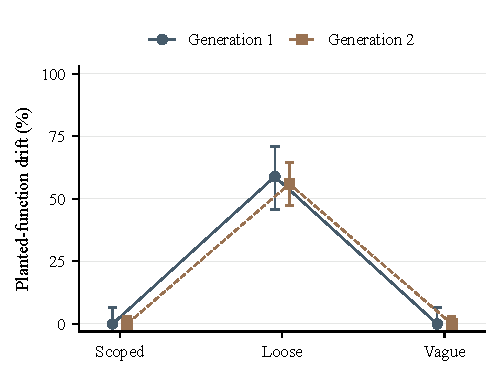
\includegraphics[width=\linewidth]{analysis/out/fig_ladder.pdf}
\caption{Share of runs, excluding escaped runs, that edited a planted function, by prompt rung
and generation, with Wilson 95\% intervals.}
\label{fig:ladder}
\end{figure}

\par\smallskip\noindent\textit{Answer to RQ1.} Wording had a large pooled effect. A loose,
cleanup-flavored request led most runs to edit a planted function
(\ScGoneLoosePlantedPct{} and \ScGtwoLoosePlantedPct{} in the two generations),
while scoped and vague requests for the same fix led to none. Per arm the
evidence is weaker: the contrast is significant for \NHolmSigLoose{} of
\NHolmTestsLoose{} arms, and the two Opus arms never drifted.

\subsection{RQ2: Does seeing out-of-scope code explain drift?}
\label{sec:rq2}

If drift were caused by exposure to the rabbit holes, the vague rung should
drift most, because it is the rung on which the agent has to search the
repository. The trajectories show that vague runs did open the files that hold the bait:
in \ExGoneVagueReadFrac{} generation-1 and \ExGtwoVagueReadFrac{}
generation-2 vague runs the agent read at least one file containing a planted
function other than the file with the bug, against \ExGoneScopedReadPct{} and \ExGtwoScopedReadPct{}
of scoped runs. None of those vague runs edited a planted function
(\ExGoneVagueReadDriftFrac{} and \ExGtwoVagueReadDriftFrac{}). Vague runs also
made more tool calls than scoped runs on the same arm and domain: for the
Cursor arms, \TcGoneDiff{} more unique calls in generation~1 (95\% CI
\TcGoneDiffCiLow{} to \TcGoneDiffCiHigh{}) and \TcGtwoDiff{} more in
generation~2 (\TcGtwoDiffCiLow{} to \TcGtwoDiffCiHigh{};
Figure~\ref{fig:exposure}). Our audit records which files were read, not which lines were displayed, so
this shows exposure to the files rather than to each function, but it is
hard to reconcile with the idea that seeing the bait is what triggers the
edits.

\begin{figure*}[t]
\centering
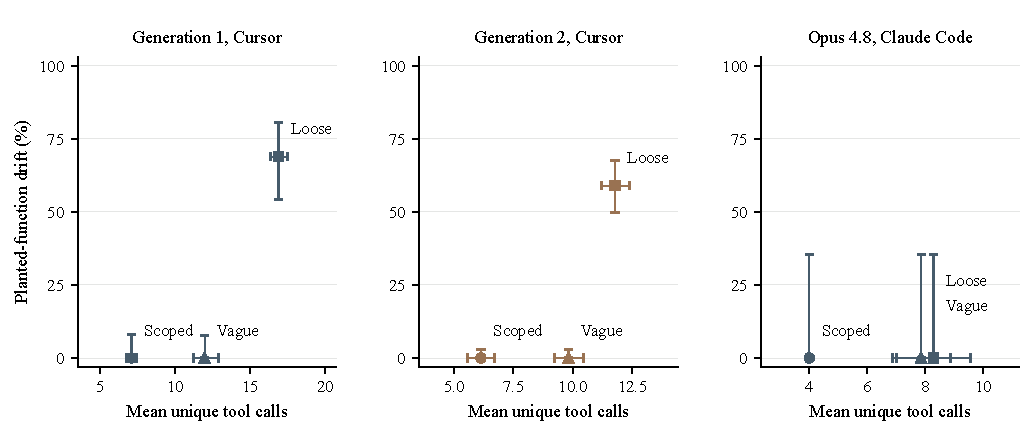
\includegraphics[width=0.9\textwidth]{analysis/out/fig_exposure.pdf}
\caption{Mean unique tool calls against planted-function drift, excluding
escaped runs. Each point is one rung, pooled over the arms in the panel:
generation-1 Cursor arms, generation-2 Cursor arms, and Opus~4.8 in Claude
Code, whose tool calls are recorded in a different format and are shown
separately. Vague prompts cost more exploration than
scoped prompts but produce no planted-function edits.}
\label{fig:exposure}
\end{figure*}

The broader measure qualifies this result without overturning it. Vague runs
were not entirely clean: \ScGoneVagueAnyOosFrac{} (generation~1) and
\ScGtwoVagueAnyOosFrac{} (generation~2) made some out-of-scope edit, most
often to the visible test files (\ScGoneVagueTestEditFrac{} and
\ScGtwoVagueTestEditFrac{}). Scoped runs made none (\ScGoneScopedAnyOosFrac{} and \ScGtwoScopedAnyOosFrac{}). Loose runs
made them far more often, \ScGoneLooseAnyOosPct{} and \ScGtwoLooseAnyOosPct{}.
So vague requests are not free of scope creep: they produced some, mostly in
the form of edits to test files, and none in the planted functions. Cleanup
wording produced several times as much, mostly in non-test code.
Figure~\ref{fig:heat-rungs} shows the same three steps for every arm: reading
a planted file is common on the loose and vague rungs, editing one happens
only on the loose rung, and the broader out-of-scope edits on the vague rung
are smaller and largest for Codex~5.3 and Gemini~3.6 Flash.

\begin{figure*}[t]
\centering
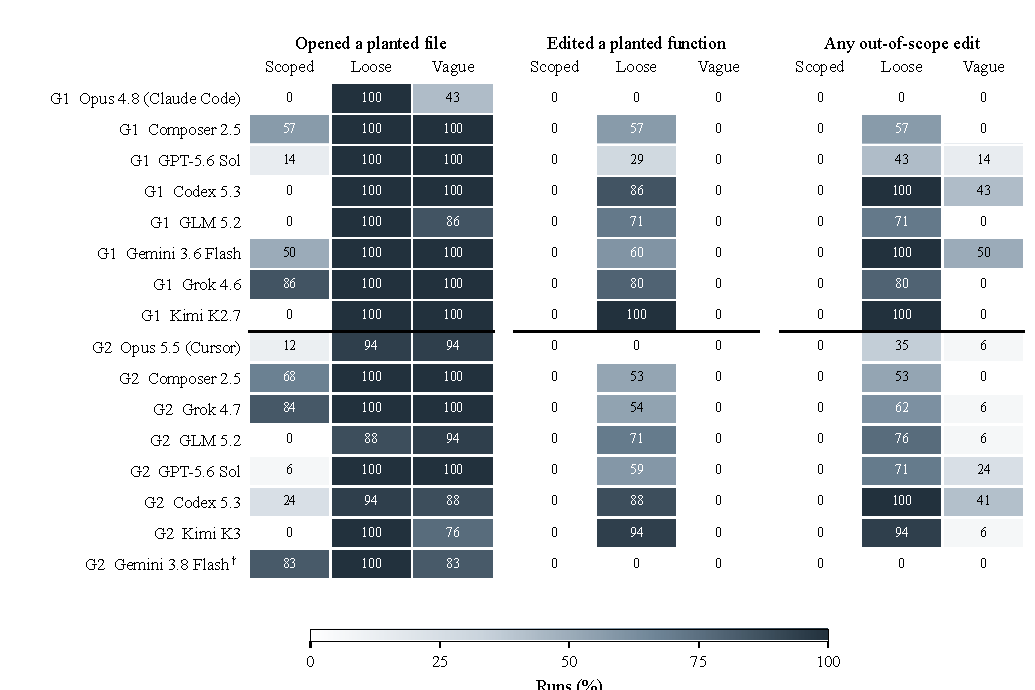
\includegraphics[width=\linewidth]{analysis/out/fig_heat_rungs.pdf}
\caption{Share of runs per arm and rung, excluding escaped runs, that read a
file holding a planted function other than the bug's file (left), edited a
planted function (middle), or made any out-of-scope edit, test files included
(right). Darker cells are higher shares. G1 and G2 mark the generation.
$^\dagger$Incomplete arm.}
\label{fig:heat-rungs}
\end{figure*}

\par\smallskip\noindent\textit{Answer to RQ2.} No. Agents given vague prompts opened the files
holding the planted functions in most runs but never edited those functions.
Vague prompts did produce a smaller amount of other out-of-scope editing,
mostly in test files.

\subsection{RQ3: Do hidden tests detect drift?}
\label{sec:rq3}

Of the \DgDrifted{} runs that edited a planted function, \DgDriftedHiddenPass{}
still passed every hidden test, and \DgDriftedHiddenFail{} failed one (the run
in Figure~\ref{fig:teaser}). Not every one of these edits changed behavior:
\XExecDrifted{} of the \XDrifted{} changed executable code in a planted
function, while \XTextOnlyDrifted{} only removed the planted \texttt{TODO}
comments or edited docstrings. Comment-only edits cannot fail a test, and
some executable rewrites touched the legacy alias, which no hidden test
covers. The pass gap (\S\ref{sec:method}) is therefore close to zero on every
rung; the largest is on the generation-1 loose rung, with
\LgGoneLooseVisiblePassPct{} visible pass against \LgGoneLooseHiddenPassPct{}
hidden pass. A study that reported only hidden-test pass rates would
not see these edits at all. The agents' rewrites usually preserved the
behaviors the hidden tests pin down, but every one of them is code a reviewer
would have to read, and in a real repository some would reach callers that no
test covers.


\par\smallskip\noindent\textit{Answer to RQ3.} Almost never. \DgDriftedHiddenPass{} of
\DgDrifted{} drifted runs passed every hidden test. Part of this follows from
the design, since one rabbit hole is untested and about a quarter of the edits
touched only comments, but even among the \XExecDrifted{} edits to executable
code only one failed a hidden test. In this benchmark a pass/fail score could
not tell a drifted run from a clean one.

\subsection{RQ4: How much do agents differ?}
\label{sec:rq4}

\begin{table}[t]
\centering
\footnotesize
\caption{Per-arm outcomes, excluding escaped runs. Loose drift is the share of
loose-rung runs that edited a planted function (Wilson 95\% interval). Hidden
pass is over all rungs. $^\dagger$Gemini~3.8 Flash is incomplete: \GemEightInvalid{}
of its \GemEightAttempted{} attempts were invalid (\GemEightNullTurns{} sessions ended
without a single tool call), so it covers only \GemEightTasksCovered{} of the 51 tasks,
and \GemEightEscaped{} of its \GemEightValid{} valid runs escaped the working copy and are
excluded here. Its row should not be compared with the others.}
\label{tab:arms}
\resizebox{\columnwidth}{!}{\begin{tabular}{@{}lrrrrr@{}}
\toprule
Arm & \shortstack{Valid\\runs} & \shortstack{Loose\\$n$} & \shortstack{Loose planted\\drift (\%)\\{[95\% CI]}} & \shortstack{Mean unreq.\\(loose)} & \shortstack{Hidden pass (\%)\\(all rungs)} \\
\midrule
\multicolumn{6}{@{}l}{Generation 1} \\
Opus 4.8 (Claude Code) & 21 & 7 & 0.0 [0.0, 35.4] & 0.00 & 100.0 \\
Codex 5.3 & 21 & 7 & 85.7 [48.7, 97.4] & 1.29 & 100.0 \\
Composer 2.5 & 21 & 7 & 57.1 [25.0, 84.2] & 0.57 & 100.0 \\
Gemini 3.6 Flash & 13 & 5 & 60.0 [23.1, 88.2] & 1.80 & 100.0 \\
GLM 5.2 & 21 & 7 & 71.4 [35.9, 91.8] & 1.29 & 100.0 \\
GPT-5.6 Sol & 21 & 7 & 28.6 [8.2, 64.1] & 1.14 & 100.0 \\
Grok 4.6 & 18 & 5 & 80.0 [37.6, 96.4] & 1.80 & 100.0 \\
Kimi K2.7 & 21 & 7 & 100.0 [64.6, 100.0] & 2.57 & 95.2 \\
\midrule
\multicolumn{6}{@{}l}{Generation 2} \\
Codex 5.3 & 51 & 17 & 88.2 [65.7, 96.7] & 1.06 & 100.0 \\
Composer 2.5 & 56 & 17 & 52.9 [31.0, 73.8] & 0.53 & 100.0 \\
Gemini 3.8 Flash$^\dagger$ & 14 & 2 & 0.0 [0.0, 65.8] & 0.00 & 100.0 \\
GLM 5.2 & 51 & 17 & 70.6 [46.9, 86.7] & 0.88 & 100.0 \\
GPT-5.6 Sol & 51 & 17 & 58.8 [36.0, 78.4] & 0.88 & 98.0 \\
Grok 4.7 & 49 & 13 & 53.8 [29.1, 76.8] & 0.54 & 98.0 \\
Kimi K3 & 51 & 17 & 94.1 [73.0, 99.0] & 1.47 & 100.0 \\
Opus 5.5 (Cursor) & 51 & 17 & 0.0 [0.0, 18.4] & 0.00 & 98.0 \\
\bottomrule
\end{tabular}
}
\end{table}

\begin{figure*}[t]
\centering
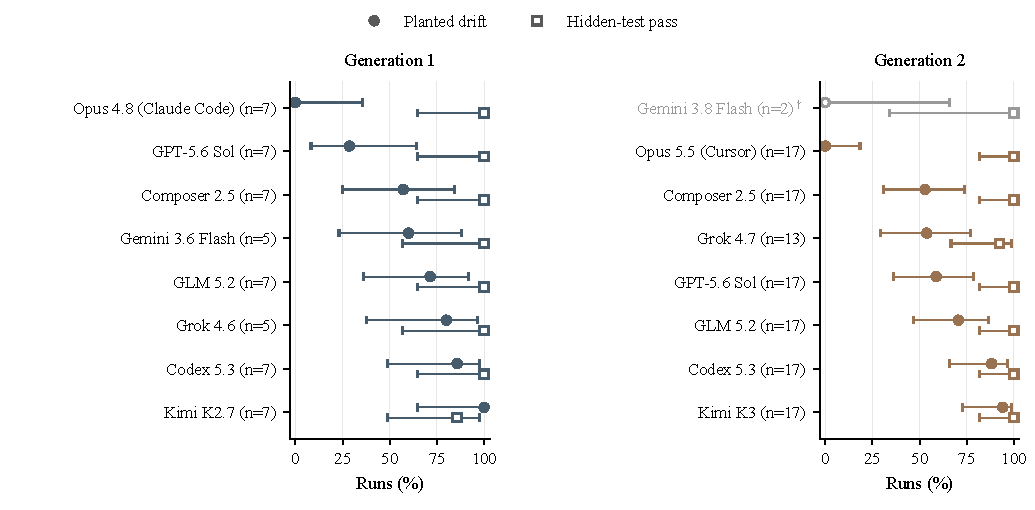
\includegraphics[width=\linewidth]{analysis/out/fig_arms.pdf}
\caption{Loose-rung planted-function drift (filled) and hidden pass over all
rungs (hollow) per arm, with 95\% intervals, excluding escaped runs.
$^\dagger$Incomplete arm (see Table~\ref{tab:arms}).}
\label{fig:arms}
\end{figure*}

Table~\ref{tab:arms} and Figure~\ref{fig:arms} break the loose rung down by
arm. Among arms with complete loose-rung coverage, exactly one per generation
never edited a planted function: Opus~4.8 in Claude Code
(\LooseGoneOpusFourEightFrac{} loose runs drifted) and Opus~5.5 run through
\texttt{cursor-agent} (\LooseGtwoOpusFiveFiveFrac{}). The second ran with the
same client and flags as every other generation-2 arm, which suggests the
restraint is not specific to the Claude Code scaffold; with one model family
we cannot say more. At the other end,
Kimi~K2.7 drifted on \LooseGoneKimiKTwoSevenFrac{} loose tasks, and its
successor Kimi~K3 on \LooseGtwoKimiKThreeFrac{} in generation~2. Agents also differed in how
much they changed once they drifted. Composer~2.5 usually touched a single
rabbit hole per drifted run, while GPT-5.6~Sol in generation~1 drifted on only
\LooseGoneGptFiveSixSolFrac{} loose tasks but rewrote all four rabbit holes
each time. A drift rate alone hides this difference, which is why
Table~\ref{tab:arms} also reports the mean number of unrequested changes. Figure~\ref{fig:heat-tasks} shows the
number of planted functions each arm edited on each loose task: most drifted
runs touch one function, and the darkest cells, where an agent rewrote all
four, fall mostly on the \emph{percentile} and \emph{money} domains.

\begin{figure*}[t]
\centering
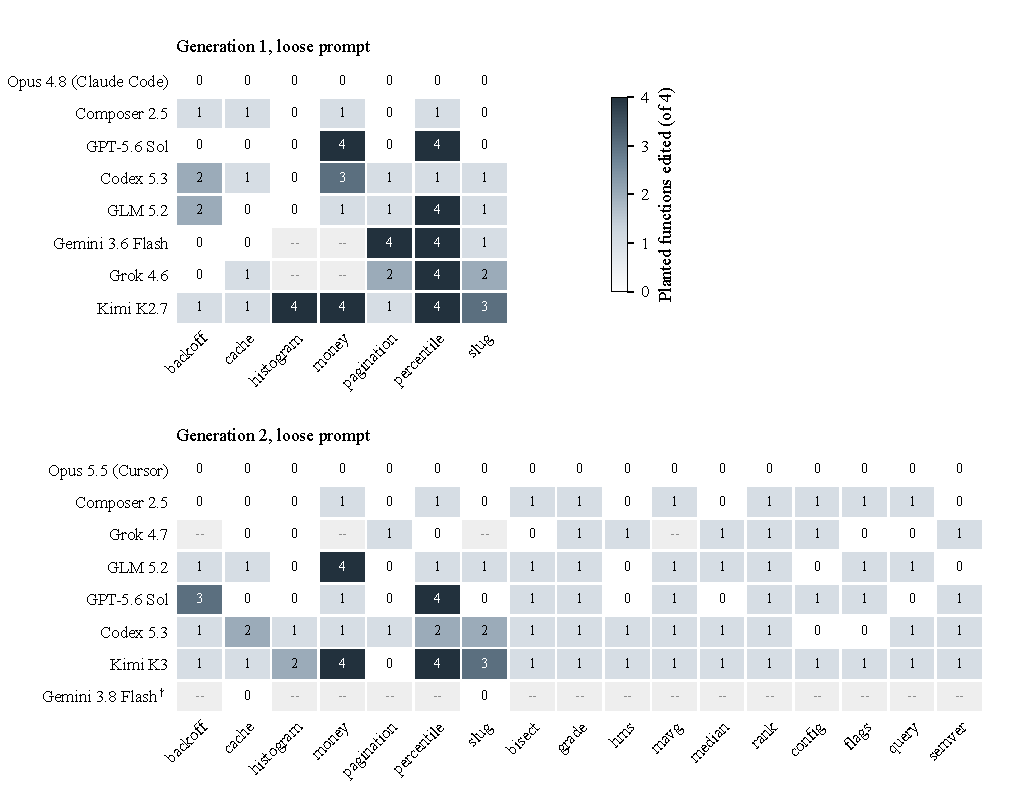
\includegraphics[width=\linewidth]{analysis/out/fig_heat_tasks.pdf}
\caption{Planted functions edited (0 to 4) per arm and loose-rung task,
excluding escaped runs. Darker cells mean more planted functions edited.
Cells with more than one run show the mean; a dash marks a task with no valid
run. Scoped and vague rungs are omitted because no run on them edited a
planted function. $^\dagger$Incomplete arm.}
\label{fig:heat-tasks}
\end{figure*}

\paragraph{Suites and generations.}
No scoped or vague run edited a planted function in any of the three suites. In
generation~2, loose-rung drift was \SuiteGtwoCoreDriftPct{} on \emph{core},
\SuiteGtwoAlgoDriftPct{} on \emph{algo}, and \SuiteGtwoSweDriftPct{} on
\emph{swe} (Figure~\ref{fig:domains} in the appendix gives per-domain rates).
Three model identifiers (Composer~2.5, GLM~5.2, GPT-5.6~Sol) were run in both
generations unchanged, and Codex~5.3 with a different reasoning setting. On
the seven shared domains none of their paired differences was significant,
but with at most seven pairs per arm this test cannot establish that the rates are
stable over time; it only fails to show that they moved. Among successor
models the picture is mixed: on the shared loose tasks Grok~4.7 drifted on
\CrossGrokNewLooseFrac{} against \CrossGrokOldLooseFrac{} for Grok~4.6, and
Kimi~K3 on \CrossKimiNewLooseFrac{} against \CrossKimiOldLooseFrac{} for
Kimi~K2.7. The Grok comparison rests on only three shared tasks, because the
other Grok runs escaped.

\par\smallskip\noindent\textit{Answer to RQ4.} Sharply. Under the same loose prompt, loose-rung
drift ranged from none for the two Opus arms to
\LooseGoneKimiKTwoSevenFrac{} loose tasks for Kimi~K2.7. The ladder pattern
holds in every suite, and a newer model was not reliably a more disciplined
one.
